\par{As the name suggests, the diagonal kernel performs operations on the diagonal elements of the matrix. 
    Table \ref{tab:lu1} summarises how the block size affects the implementation of the diagonal kernel.}

\begin{table}[!h]
    \centering
    \begin{tabular}{| l | l | l | l |}
    \hline
    \emph{Block Size} & \emph{Data Block} & \emph{\#Work Groups} & \emph{\#Work-Items / Work-Group} \\ \hline
    2 & 2x2 & 1 & 2 \\ \hline
    4 & 4x4 & 1 & 4 \\ \hline
    8 & 8x8 & 1 & 8 \\ \hline
    16 & 16x16 & 1 & 16 \\ \hline
    32 & 32x32 & 1 & 32 \\ \hline
    64 & 64x64 & 1 & 64\\ \hline
    \end{tabular}
    \caption{rory blah blah.}
    \label{tab:lu1}
\end{table}

\par{The first point to note is that the diagonal kernel is clearly not optimised for parallel computing. 
    In OpenCL, the work-groups are scheduled in parallel on each thread of the Xeon Phi and Xeon CPU. 
    In this case, the number of work-groups is always one. For example, on the Xeon Phi, 
    the entire computation of the diagonal kernel would take place on just one of the 240 hardware threads.}

\par{Although there is no parallelism between threads in this case, implicit SIMD vectorisation of work-items is supported 
    by the OpenCL compiler. However, this requires both that kernels be as simple as possible and that they execute the same 
    instructions. This is not the case with this kernel. The algorithm is such that each work-item carries out a different 
    number of floating point operations, depending on its ID. This renders instruction-level parallelism impossible in this case. 
    Figure \ref{FlopCount} shows that, for a work-group of 16 work-items, the number of floating point operations varies according to 
    the ID of the work-item. In fact, the first work-item of every work-group does no computation whatsoever.}

\begin{figure}[!h]
    \centering
    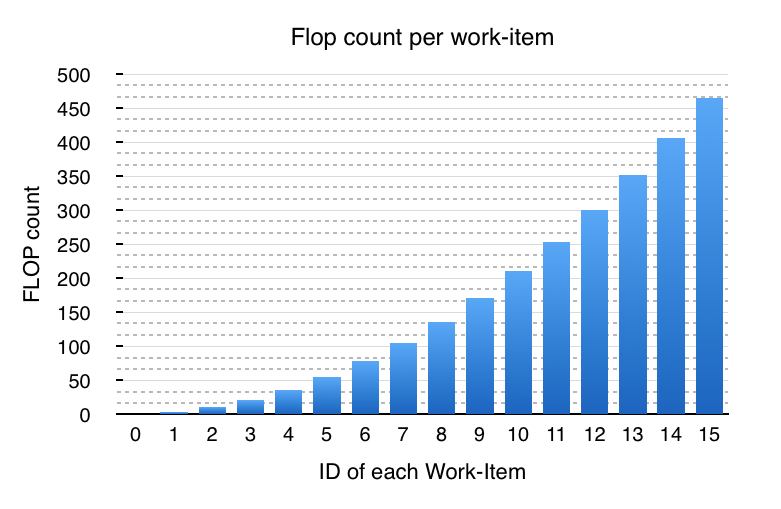
\includegraphics[width=0.6\textwidth]{figures/FlopCount.png}
    \caption{Rory blah blah blah.}
    \label{FlopCount}
\end{figure}

\par{Figure \ref{DiagonalKernel} illustrates a number of important points. It is clear that, 
    out of the three devices used, the Xeon Phi shows the worst performance. 
    Achieving high-performance with the Xeon Phi requires that work-items be vectorised and 
    that large numbers of work-groups be scheduled in parallel. Neither such condition is satisfied in this case. 
    It is interesting to note that the Xeon CPU performs best with an algorithm of low parallelism. 
    Undoubtedly, the CPU’s support for out-of-order execution gives it an advantage over the Xeon Phi, 
    which supports in-order execution only.}

\begin{figure}[!h]
    \centering
    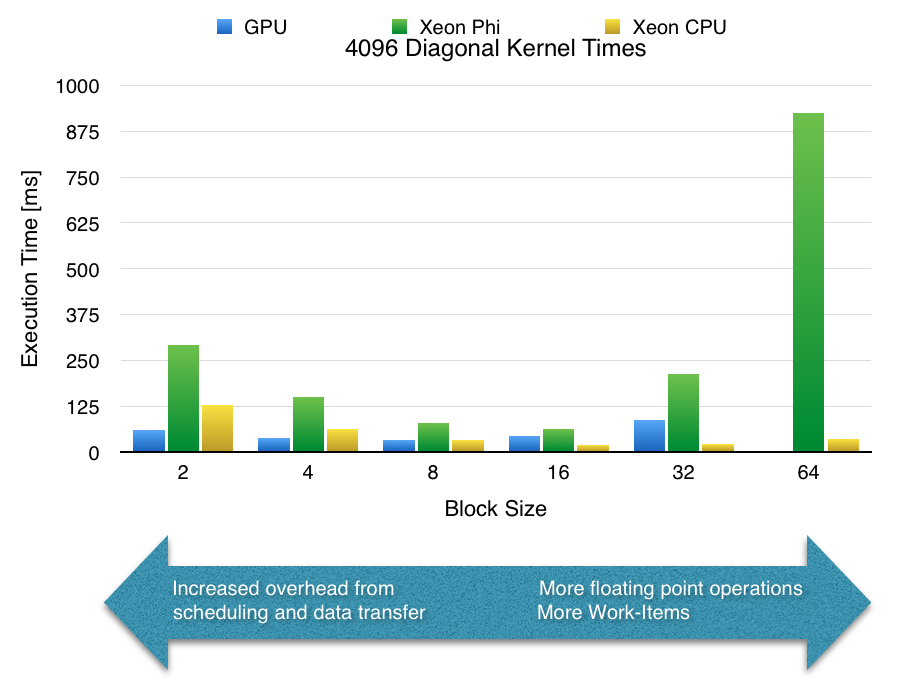
\includegraphics[width=0.6\textwidth]{figures/DiagonalKernel.png}
    \caption{Rory blah blah blah.}
    \label{DiagonalKernel}
\end{figure}

\par{The GPU also achieves good performance compared to the Xeon Phi. Unlike on the Xeon CPU and Xeon Phi, 
    the work-items are scheduled in parallel in the warps of the GPU. It does not suffer the same lack of 
    performance as a result of having only 1 work-group.}



